\documentclass[10pt,aspectratio=169]{beamer}
\graphicspath{ {images/} }
% --- pdflatex-safe font & micro-typography ---
\usepackage[T1]{fontenc}
\usepackage[utf8]{inputenc}
\usepackage{lmodern}
\usepackage{microtype}

\usepackage{tikz}
\usetikzlibrary{arrows.meta}

% --- math & symbols ---
\usepackage{amsmath,amssymb,mathtools,bm}

% --- hyperlinks (Beamer already loads hyperref; this is safe) ---
\hypersetup{hidelinks}

% --- theme ---
\usetheme[numbering=fraction]{metropolis}

\usepackage{pgfpages} % for notes layouts

% --- bibliography ---
\usepackage[round,authoryear]{natbib}

% --- Choose ONE of these toggles when compiling ---
% \setbeameroption{hide notes}                        % audience version (default)
% \setbeameroption{show notes}                        % notes printed under each slide
% \setbeameroption{show only notes}                   % notes-only PDF (for printing)
% \setbeameroption{show notes on second screen=right} % slide + notes side-by-side

% --- shortcuts ---
\newcommand{\E}{\mathbb{E}}
\newcommand{\R}{\mathbb{R}}
\newcommand{\btheta}{\boldsymbol{\theta}}
\newcommand{\bx}{\boldsymbol{x}}
\setbeamercovered{transparent}
% --- title info ---
\title{Training dynamics of overparameterized neural networks}
\subtitle{Overview of results}
\author{Shreyas Kalvankar}
\institute{TU Delft}
\date{\today}

\begin{document}

\maketitle

% -----------------------------------------------------------
% SETUP SLIDE
% -----------------------------------------------------------
\begin{frame}{Problem setup}

	We study regression on the unit circle
	\[
		S^1 \simeq [0,2\pi),
		\qquad
		x(\gamma)=(\cos\gamma,\sin\gamma).
	\]

	The target is a finite Fourier mixture:
	\[
		f^\star(\gamma)
		=
		a_0
		+
		\sum_{k=1}^{K}
		\left(
		a_k\cos(k\gamma)
		+
		b_k\sin(k\gamma)
		\right).
	\]

	\medskip

	\textbf{Question:}
	which Fourier components are learned quickly, and what changes at finite sample size and finite width?

	\note{
		Start from the concrete setting. I chose \(S^1\) because frequency is literal here.
		The Fourier basis gives a clean way to study spectral bias.
		The goal is not to explain all neural networks, but to analyze one setting where the learning operator can be written explicitly.
	}

\end{frame}

% -----------------------------------------------------------
% TRAINING DYNAMICS SLIDE
% -----------------------------------------------------------
\begin{frame}{Training dynamics}

	Consider a one-hidden-layer ReLU network
	\[
		f_\theta(x) = \frac{1}{\sqrt m} \sum_{\alpha=1}^{m} v_\alpha\,\sigma(w_\alpha^\top x+b_\alpha), \qquad x\in S^1,
	\]
	where \(\theta = \{(v_\alpha, w_\alpha, b_\alpha)\}_{\alpha=1}^m$,
		initialized via $v_\alpha, w_\alpha \sim \mathcal{N}(0, 1)$ and $b_\alpha =
	0\) denotes the set of trainable parameters.

	\pause
	We train with squared loss in continuous time:
	\[
		\mathcal L(\theta)
		=
		\frac12
		\|f_\theta-f^\star\|_{L^2(S^1)}^2 .
	\]

	\pause

	Define the residual
	\[
		r_t(x)=f_{\theta_t}(x)-f^\star(x).
	\]

\end{frame}

% -----------------------------------------------------------
% NTK DERIVATION SLIDE
% -----------------------------------------------------------
\begin{frame}{From parameter flow to the tangent kernel}

	Gradient flow in parameter space is
	\[
		\frac{d}{dt}\theta_t
		=
		-\nabla_\theta \mathcal L(\theta_t).
	\]

	\pause
	Since
	\[
		\mathcal L(\theta)
		=
		\frac12
		\int_{S^1}
		\bigl(f_\theta(y)-f^\star(y)\bigr)^2
		\,d\mu(y),
	\]
	\pause
	we have
	\[
		\nabla_\theta \mathcal L(\theta_t)
		=
		\int_{S^1}
		r_t(y)\,\nabla_\theta f_{\theta_t}(y)
		\,d\mu(y).
	\]

	\pause
	Using the chain rule, for fixed \(x\),
	\[
		\frac{d}{dt} f_{\theta_t}(x)
		=
		\left\langle
		\nabla_\theta f_{\theta_t}(x),
		\dot\theta_t
		\right\rangle
		= \left\langle \nabla_\theta f{\theta_t}(x), -\nabla_\theta \mathcal L(\theta_t) \right\rangle.
	\]

	\pause
	Substituting the gradient flow gives
	\[
		\frac{d}{dt} f_{\theta_t}(x)
		=
		-
		\int_{S^1}
		\underbrace{
			\left\langle
			\nabla_\theta f_{\theta_t}(x),
			\nabla_\theta f_{\theta_t}(y)
			\right\rangle
		}_{\Theta_t(x,y)}
		r_t(y)
		\,d\mu(y).
	\]

	\note{
		This is the point where the neural tangent kernel appears naturally.
		It is not introduced as an arbitrary kernel. It is the Gram kernel of the parameter gradients of the network output.
		The important object is the inner product between how the output at \(x\) and the output at \(x'\) change under infinitesimal parameter perturbations.
	}

\end{frame}

% -----------------------------------------------------------
% NTK OPERATOR SLIDE
% -----------------------------------------------------------
\begin{frame}{Residual dynamics in function space}

	The neural tangent kernel is
	\[
		\Theta_t(x,y)
		=
		\left\langle
		\nabla_\theta f_{\theta_t}(x),
		\nabla_\theta f_{\theta_t}(y)
		\right\rangle .
	\]

	\pause
	Define an integral operator
	\[
		(T_t g)(x)
		=
		\int_{S^1}
		\Theta_t(x,y)g(y)\,d\mu(y).
	\]

	\pause
	Thus,
	\[
		\frac{d}{dt} r_t(x)
		=
		\frac{d}{dt} f_{\theta_t}(x)
		=
		-
		\int_{S^1}
		\Theta_t(x,y)
		r_t(y)
		\,d\mu(y).
		=
		-T_t r_t
	\]

	If \(T_t\equiv T\) is fixed, then
	\[
		r_t
		=
		e^{-tT}r_0.
	\]

	So the decay of \(r_t\) is determined by the spectrum of \(T\).

	\note{
		This is the main function-space formulation.
		The original optimization problem is nonlinear in the parameters.
		But the residual evolves by an operator \(T_t\) in function space.
		At finite width, \(T_t\) changes with time.
		In the infinite-width NTK limit, it becomes fixed, which gives the clean reference dynamics.
	}

\end{frame}

% -----------------------------------------------------------
% INFINITE-WIDTH LIMITING KERNEL SLIDE
% -----------------------------------------------------------
\begin{frame}{Infinite-width NTK reference}

	At finite width, the tangent kernel is an empirical average over neurons:
	\[
		\Theta_t^{(m)}(x,y)
		=
		\frac{1}{m}
		\left\langle \nabla_\theta f_\theta(x), \nabla_\theta f_\theta(y) \right\rangle
	\]

	\pause
	Taking limit \(m\to\infty\),
	\[
		\Theta_t^{(m)}(x,y)
		\longrightarrow
		\Theta_t^{(\infty)}(x,y)
		= 		\E_{\theta_0}
		\left[
			\left\langle
			\nabla_\theta f_{\theta_0}(x),
			\nabla_\theta f_{\theta_0}(y)
			\right\rangle
			\right].
	\]
	and the limit stays fixed during training:
	\[
		\Theta_t^{(\infty)}
		\approx
		\Theta_0^{(\infty)}
		\approx
		\Theta_\infty.
	\]

	\pause
	On \(S^1\), write \(x=x(\gamma)\), \(y=x(\psi)\), and
	\[
		\delta = |\gamma-\psi|, \qquad \delta\in[0,\pi].
	\]
	Then
	\[
		\Theta_\infty(x(\gamma),x(\psi))
		=
		\Theta(\delta)
		=
		\frac{1}{2\pi}
		\Bigl(
		\sin\delta
		+
		2(\pi-\delta)\cos\delta
		+
		(\pi-\delta)
		\Bigr).
	\]

	\note{
		The key point is that finite-width kernels are empirical averages over neurons.
		At initialization, the infinite-width kernel is the expectation of one-neuron tangent contributions.
		In the NTK regime, parameter movement per neuron becomes small enough that the tangent kernel stays fixed during training.
		On the circle, the limiting kernel depends only on the angular distance \(\delta\).
		This prepares the next slide: dependence only on angular difference means the operator is a convolution operator.
	}

\end{frame}

% -----------------------------------------------------------
% SPECTRAL BIAS SLIDE
% -----------------------------------------------------------
\begin{frame}{Spectral bias in the continuum reference model}

	Since \(\Theta_\infty(x(\gamma),x(\psi))=\Theta(\gamma-\psi)\), the operator is a convolution:
	\[
		(T_\infty g)(\gamma)
		=
		\int_{0}^{2\pi}
		\Theta(\gamma-\psi)\,g(\psi)\,\frac{d\psi}{2\pi}.
	\]

	\pause
	Therefore the Fourier basis diagonalizes \(T_\infty\):
	\[
		T_\infty \phi_p
		=
		\lambda_p \phi_p.
	\]

	\pause
	Write the residual as
	\[
		r_t
		=
		\sum_p \alpha_p(t)\phi_p.
	\]

	Then
	\[
		\frac{d}{dt}\alpha_p(t)
		=
		-\lambda_p\alpha_p(t),
		\qquad
		\alpha_p(t)
		=
		e^{-\lambda_p t}\alpha_p(0).
	\]

	\pause
	\textbf{Spectral bias:}
	modes with larger \(\lambda_p\) decay faster.
	\begin{tikzpicture}[remember picture, overlay]
		\node<4->[anchor=south east, xshift=-1.0cm, yshift=2.5cm]
		at (current page.south east)
		{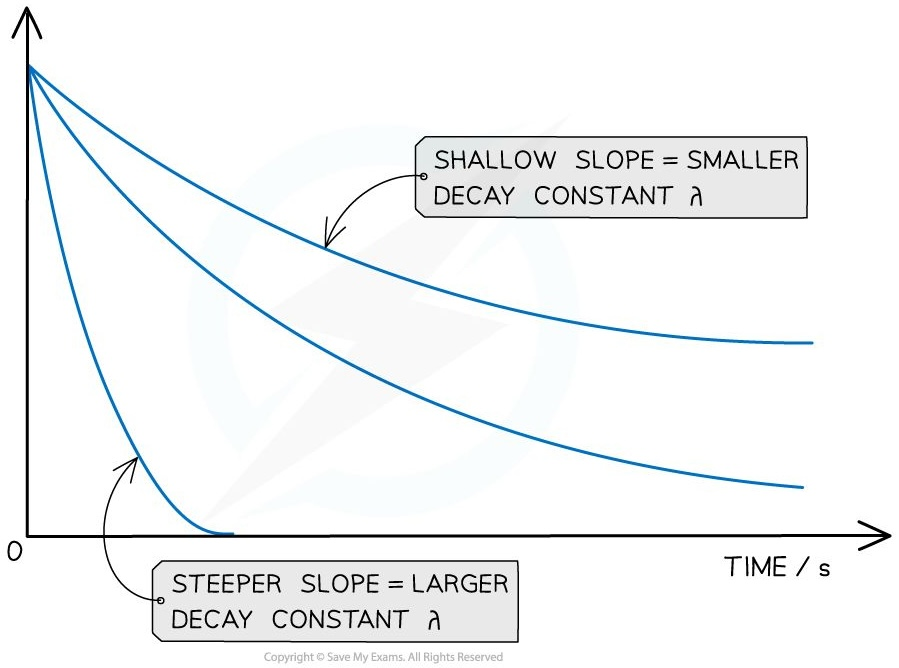
\includegraphics[width=4.5cm]{decay}};
	\end{tikzpicture}


	\note{
		This is the cleanest point of the whole setup.
		Because the limiting kernel depends only on angular distance, the operator is a convolution operator.
		Fourier modes are eigenfunctions of convolution operators.
		Once the residual is expanded in that eigenbasis, each coefficient follows a scalar ODE.
		So spectral bias is not a vague statement here: it is an eigenvalue statement.
		The learning speed of each Fourier mode is exactly controlled by the corresponding eigenvalue of the NTK integral operator.
	}

\end{frame}

\begin{frame}{Spectral bias}

	\begin{tikzpicture}[remember picture, overlay]
		\node[
			anchor=south east,
			xshift=-1.0cm,
			yshift=1.0cm
		]
		at (current page.south east)
		{
			\begin{minipage}{\textwidth}
				\centering
				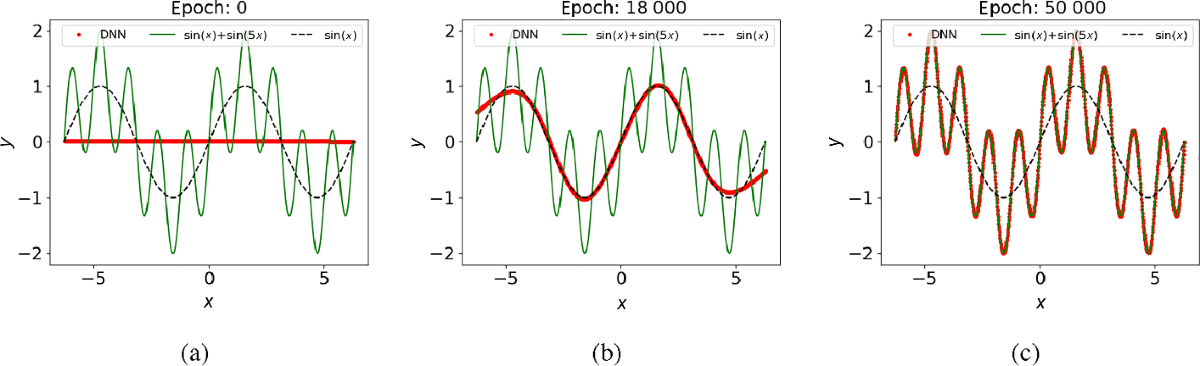
\includegraphics[width=\textwidth]{spectral-bias}

				\vspace{0.1cm}
				{\scriptsize Image source: \emph{Overview of Spectral Bias in Deep Learning}, Vol. 7}
			\end{minipage}
		};
	\end{tikzpicture}

\end{frame}
% -----------------------

% -----------------------------------------------------------
% RESEARCH QUESTION SLIDE
% -----------------------------------------------------------
\begin{frame}{Main research question}

	\textbf{Ideal reference:}
	\[
		\frac{d}{dt}r_t=-T_\infty r_t,
		\qquad
		T_\infty\phi_p=\lambda_p\phi_p.
	\]

	\pause
	\textbf{Question:}

	\medskip

	How much of this Fourier-diagonal picture survives when we move away from the idealized setting?

	\pause
	\begin{enumerate}
		\item finite samples \(n\)
		\item finite width \(m\)
	\end{enumerate}

	\note{
		This slide transitions from the clean continuum reference model to the actual thesis contributions.
		The main question is not whether spectral bias exists in the ideal model; that follows from the spectrum.
		The thesis asks whether this spectral picture survives under finite-sample and finite-width perturbations.
		The first two parts are controlled perturbation results.
		The evolving-kernel part is empirical and more exploratory.
	}

\end{frame}

\begin{frame}{Finite samples}

	Sample points:
	\[
		\gamma_1,\ldots,\gamma_n \sim \mathrm{Unif}[0,2\pi).
	\]
	Restrict to
	\[
		\mathcal H_K=\mathrm{span}\{1,\sqrt{2}\cos\gamma,\sqrt{2}\sin\gamma,\ldots,
		\sqrt{2}\cos K\gamma,\sqrt{2}\sin K\gamma\}.
	\]

	\pause
	Collect sampled Fourier features in
	\[
		\Phi_{i,p}=\phi_p(\gamma_i),
		\qquad
		\Phi\in\mathbb R^{n\times (2K+1)}.
	\]

	Let \(A\in\mathbb R^{n\times n}\) be the normalized sampled kernel matrix:
	\[
		A_{ij}
		=
		\frac1n\Theta(\gamma_i-\gamma_j).
	\]

	\pause
	We wish to find how do these behave,
	\[
		G=\frac1n\Phi^\top\Phi,
		\qquad
		H=\frac1n\Phi^\top A\Phi .
	\]


\end{frame}

\begin{frame}{Finite samples}

	With high probability,
	\[
		G\approx I,
		\qquad
		H\approx \Lambda^{(n)}.
	\]

	\textbf{Meaning:} finite sampling perturbs the Fourier-diagonal picture, but on fixed \(H_K\), Fourier modes are
	almost orthogonal and decay rates are still governed by the continuum eigenvalues.

\end{frame}

\begin{frame}{Proof idea: entrywise concentration}

	\begin{columns}[T,onlytextwidth]

		\begin{column}{0.48\textwidth}
			\textbf{Gram matrix \(G\)}
			\[
				G_{pq}
				=
				\frac1n\sum_{i=1}^{n}
				\phi_p(\gamma_i)\phi_q(\gamma_i).
			\]

			\[
				\E[G_{pq}]=\delta_{pq}.
			\]

			\medskip
			Entry = average of independent bounded variables.

			\[
				\Rightarrow \text{Bernstein}
			\]
		\end{column}

		\begin{column}{0.48\textwidth}
			\textbf{Compressed operator \(H\)}
			\[
				H_{pq}
				=
				\frac{1}{n^2}
				\sum_{i,j=1}^{n}
				\phi_p(\gamma_i)
				\Theta(\gamma_i-\gamma_j)
				\phi_q(\gamma_j).
			\]

			\[
				\E[H_{pq}]
				=
				\lambda_p^{(n)}\delta_{pq}.
			\]

			\medskip
			Changing one sample changes only \(O(n)\) terms.

			\[
				\Rightarrow \text{McDiarmid}
			\]
		\end{column}

	\end{columns}

	\pause
	\vspace{0.25cm}

	Apply the inequality entrywise, then union bound over all \(p,q\):
	\[
		G\approx I,
		\qquad
		H\approx \Lambda^{(n)}.
	\]

	\medskip

	\textbf{Consequence:} the sampled operator remains approximately Fourier-diagonal on the subspace.

\end{frame}

\begin{frame}{Empirical finite-sample concentration}

	\begin{columns}[T,onlytextwidth]

		\begin{column}{0.49\textwidth}
			\centering
			
\includegraphics[width=\textwidth]{theory_envelope_compare_gram_err_max}

			\vspace{0.1cm}
			{\scriptsize Gram matrix concentration: \(\|G-I\|_{\max}\)}
		\end{column}

		\begin{column}{0.49\textwidth}
			\centering
			
\includegraphics[width=\textwidth]{theory_envelope_compare_comp_err_max}

			\vspace{0.1cm}
			{\scriptsize Compressed operator concentration: \(\|H-\Lambda^{(n)}\|_{\max}\)}
		\end{column}

	\end{columns}

	\note{
		This slide is the empirical counterpart of the concentration argument.
		The left plot shows that the sampled Fourier geometry becomes closer to orthonormal as the number of samples grows.
		The right plot shows the same kind of concentration for the compressed operator.
		The green curve is the theoretical envelope, while the empirical means and 95 percent quantiles are much smaller.
		So the theory is conservative, but it captures the right decay trend.
	}

\end{frame}

% -----------------------------------------------------------
% FINITE-SAMPLE MODE DYNAMICS SLIDE
% -----------------------------------------------------------
\begin{frame}{Finite-sample dynamics: observed vs diagonal prediction}

	\vspace{-0.2cm}

	\centering

	
\includegraphics[
		width=0.92\textwidth,
		height=0.36\textheight,
		keepaspectratio
	]{story_02_random_n4096_components_first200.png}

	\vspace{0.15cm}

	
\includegraphics[
		width=0.92\textwidth,
		height=0.36\textheight,
		keepaspectratio
	]{story_02_random_n4096_components_all_steps_high_freq_only.png}

	\vspace{0.1cm}

	{\scriptsize
		Top: early dynamics for all retained components.
		Bottom: later dynamics for higher-frequency components.
	}

	\note{
		This slide connects the finite-sample concentration result to actual training dynamics.
		If the sampled Fourier modes were exact eigenvectors, each normalized coefficient would follow the dashed exponential prediction.
		In the first 200 steps, the observed curves closely follow the diagonal prediction.
		Over longer time scales, deviations become visible, especially once some components have decayed close to the numerical or finite-sample error floor.
		The point is not that the sampled dynamics are exactly diagonal forever, but that the finite-sample Fourier approximation accurately explains the early and intermediate dynamics.
	}

\end{frame}

% -----------------------------------------------------------
% PRECONDITIONING SLIDE
% -----------------------------------------------------------
\begin{frame}{Using the spectrum for preconditioning}

	\centering

	
\includegraphics[
		width=0.95\textwidth,
		height=0.63\textheight,
		keepaspectratio
	]{all_mode_decay_three_panel_mean_std_n4096.png}

	\vspace{0.15cm}

	\begin{minipage}{0.88\textwidth}
		\small
		Based on the sampled spectral picture, we can ask whether the dynamics can be
		preconditioned so that all modes in \(\mathcal H_K\) decay on a comparable time scale.

		\medskip

		\textbf{Theory preconditioner:} uses only the predicted eigenvalues
		\(\lambda_p^{(n)}\).

		\textbf{Empirical preconditioner:} uses the observed sampled operator.
	\end{minipage}

	\note{
		This is a consequence of understanding the sampled Fourier dynamics.
		In the baseline dynamics, different modes decay at very different rates because their eigenvalues are different.
		If we know the eigenvalue structure, we can try to rescale the update so that the retained modes decay at comparable rates.
		The middle panel shows a theory preconditioner, which only uses the predicted finite-sample eigenvalues.
		The right panel shows an empirical preconditioner, which uses the sampled operator itself.
		The point is not to propose this as a practical optimizer, but to show that the spectral analysis gives actionable control over the dynamics in the low-frequency subspace.
	}

\end{frame}

% -----------------------------------------------------------
% PRECONDITIONING VS SAMPLE SIZE SLIDE
% -----------------------------------------------------------
\begin{frame}{Increasing sample size improves theory-based preconditioning}

	\centering

	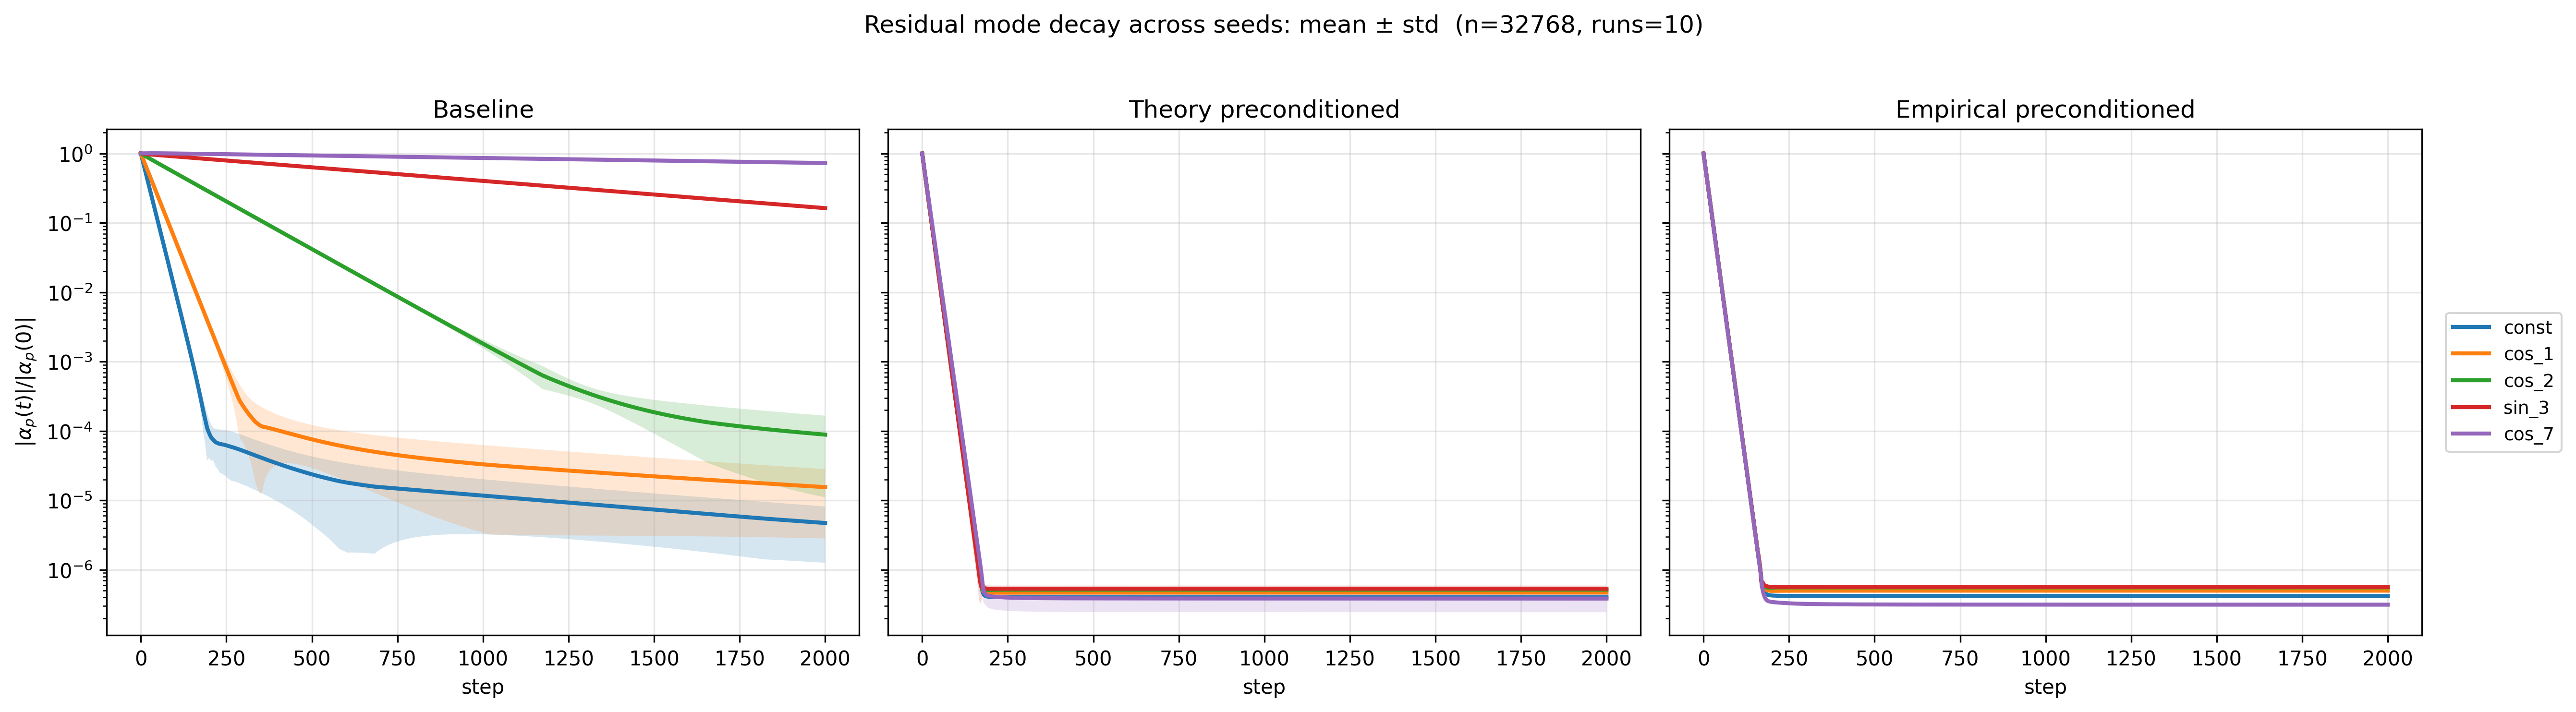
\includegraphics[
		width=0.95\textwidth,
		height=0.63\textheight,
		keepaspectratio
	]{all_mode_decay_three_panel_mean_std_n32768.png}

	\vspace{0.15cm}

	\begin{minipage}{0.88\textwidth}
		\small
		Keeping the same setup but increasing the sample size improves the spectral estimate,
		so the theory-based preconditioner gets closer to the empirically preconditioned one.

		\medskip

		\textbf{Takeaway:} as \(n\) increases, the finite-sample eigenvalue prediction becomes more accurate,
		and preconditioning based only on \(\Lambda^{(n)}\) becomes nearly as effective as using the empirical operator.
	\end{minipage}

	\note{
		This slide has exactly the same interpretation as the previous one, but at a larger sample size.
		The key comparison is between the middle and right panels.
		For \(n=4096\), theory-based preconditioning already works well, but there is still a visible gap to the empirical preconditioner.
		When we increase to \(n=32768\), that gap becomes much smaller.
		This is consistent with the finite-sample concentration results:
		as the sampled operator gets closer to its predicted Fourier-diagonal form, a preconditioner based only on the predicted eigenvalues becomes nearly optimal on the retained subspace.
	}

\end{frame}

% -----------------------------------------------------------
% FINITE-WIDTH SETUP SLIDE
% -----------------------------------------------------------
\begin{frame}{Finite width: frozen operator at initialization}

	Now keep the input space continuous, but use finite width \(m\).

	\[
		T_0^{(m)}
		=
		\frac1m
		\sum_{r=1}^{m}
		T^{(r)} .
	\]

	Here \(T^{(r)}\) is the one-neuron tangent operator at initialization.

	\pause
	Let \(P_K: L^2(S^1) \to \mathcal H_K\) be an orthogonal projection.
	Project to the retained Fourier subspace:
	\[
		B_m^{(K)}
		=
		P_KT_0^{(m)}P_K,
		\qquad
		\Lambda_K
		=
		P_KT_\infty P_K .
	\]

	\pause
	For Fourier modes \(\phi_p,\phi_q\),
	\[
		(B_m^{(K)})_{pq}
		=
		\frac1m
		\sum_{r=1}^{m}
		\xi_{r,pq},
		\qquad
		\xi_{r,pq}
		=
		\langle \phi_p,T^{(r)}\phi_q\rangle .
	\]

	\note{
		This slide sets up the finite-width frozen result.
		Unlike the finite-sample part, the circle is still continuous.
		The randomness now comes only from the initialized neurons.
		The main structural point is that the frozen finite-width operator is an average over one-neuron operators.
		After projection to \(\mathcal H_K\), each matrix entry becomes an empirical average over neurons.
	}

\end{frame}

% -----------------------------------------------------------
% FINITE-WIDTH CONCENTRATION SLIDE
% -----------------------------------------------------------
\begin{frame}{Finite width: concentration around the infinite-width block}

	Since the neurons are i.i.d.,
	\[
		\mathbb E[B_m^{(K)}]
		=
		\Lambda_K .
	\]

	\pause
	Each entry is an average of independent one-neuron contributions:
	\[
		(B_m^{(K)})_{pq}
		-
		(\Lambda_K)_{pq}
		=
		\frac1m
		\sum_{r=1}^{m}
		\Bigl(
		\xi_{r,pq}
		-
		\mathbb E\xi_{r,pq}
		\Bigr).
	\]

	\pause
	The variables are not bounded, but Gaussian initialization gives sub-exponential tails.

	\[
		\xi_{r,pq}
		\quad
		\text{sub-exponential}
	\]

	\pause
	Bernstein plus a union bound gives
	\[
		\|B_m^{(K)}-\Lambda_K\|_{\max}
		\lesssim
		\sqrt{\frac{\log d_K}{m}}
		\qquad
		\text{with high probability.}
	\]

	\note{
		This is the concentration step.
		The expectation is the infinite-width block because averaging one-neuron tangent contributions gives the limiting NTK operator.
		The concentration argument is entrywise.
		The only difference from the finite-sample Gram result is that the one-neuron variables are not bounded, since the weights are Gaussian.
		They are instead sub-exponential, which is enough for Bernstein.
		After applying Bernstein to each entry, we union bound over the \(d_K^2\) entries.
	}

\end{frame}

% -----------------------------------------------------------
% FINITE-WIDTH EMPIRICAL CONCENTRATION SLIDE
% -----------------------------------------------------------
\begin{frame}{Empirical finite-width concentration}

	\centering

	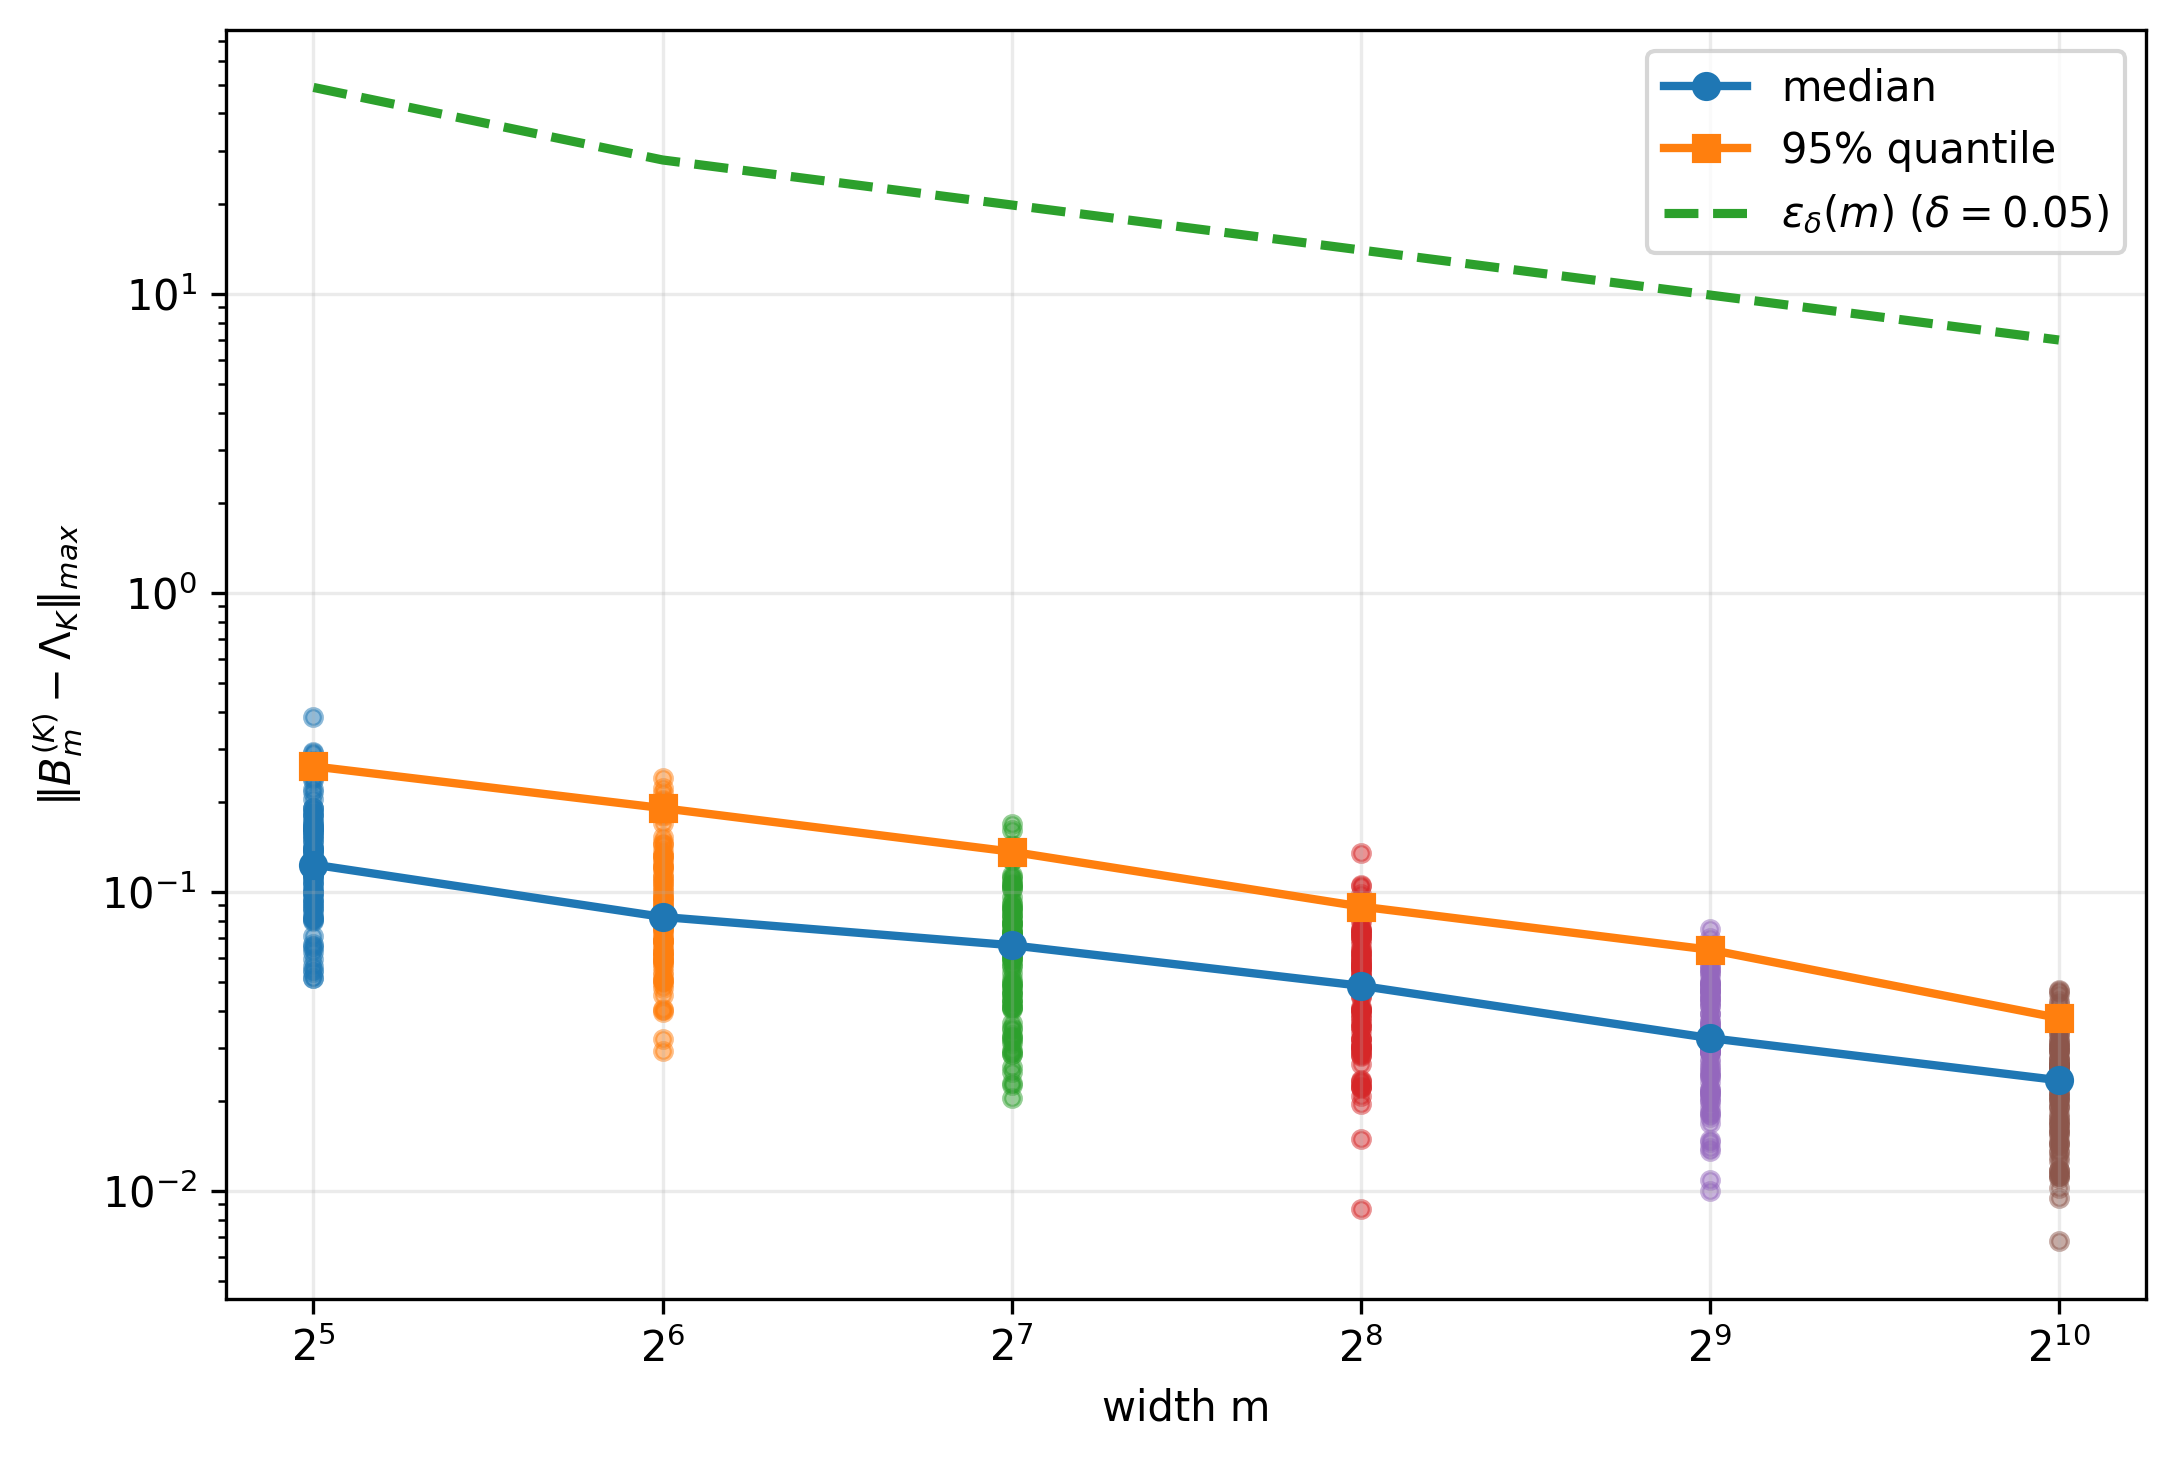
\includegraphics[
		width=0.78\textwidth,
		height=0.62\textheight,
		keepaspectratio
	]{03_concentration_B_m}

	\vspace{0.15cm}

	\begin{minipage}{0.86\textwidth}
		\small
		The bound is conservative because it is proved entrywise, uses a uniform tail bound
		for all Fourier pairs, and then applies a union bound over the whole \(d_K\times d_K\)
		block.

		It also controls worst-case high-probability behavior, not the typical median behavior.
	\end{minipage}

	\note{
		The important point here is why the theoretical envelope is loose.
		First, the proof bounds every matrix entry separately instead of using the structure of the full matrix.
		Second, it uses a worst-case sub-exponential tail estimate for the one-neuron contributions.
		Third, after obtaining an entrywise bound, it pays a union-bound cost over all Fourier-coordinate pairs.
		I wasn't able to figure out a better way to improve on this.
	}

\end{frame}

% -----------------------------------------------------------
% FOURIER-PLANE ALIGNMENT SLIDE
% -----------------------------------------------------------
\begin{frame}{Finite-width eigenspaces vs Fourier planes}

	\begin{columns}[T,onlytextwidth]

		\begin{column}{0.47\textwidth}
			For each frequency \(k\geq 1\), the relevant continuum eigenspace is the
			two-dimensional Fourier plane
			\[
				\mathcal F_k
				=
				\mathrm{span}\{\phi_{k,c},\phi_{k,s}\}.
			\]

			At finite width, we compare this with the matched empirical eigenspace
			\[
				\widehat{\mathcal F}_k^{(m)}.
			\]

		\end{column}

		\begin{column}{0.51\textwidth}
			\centering
			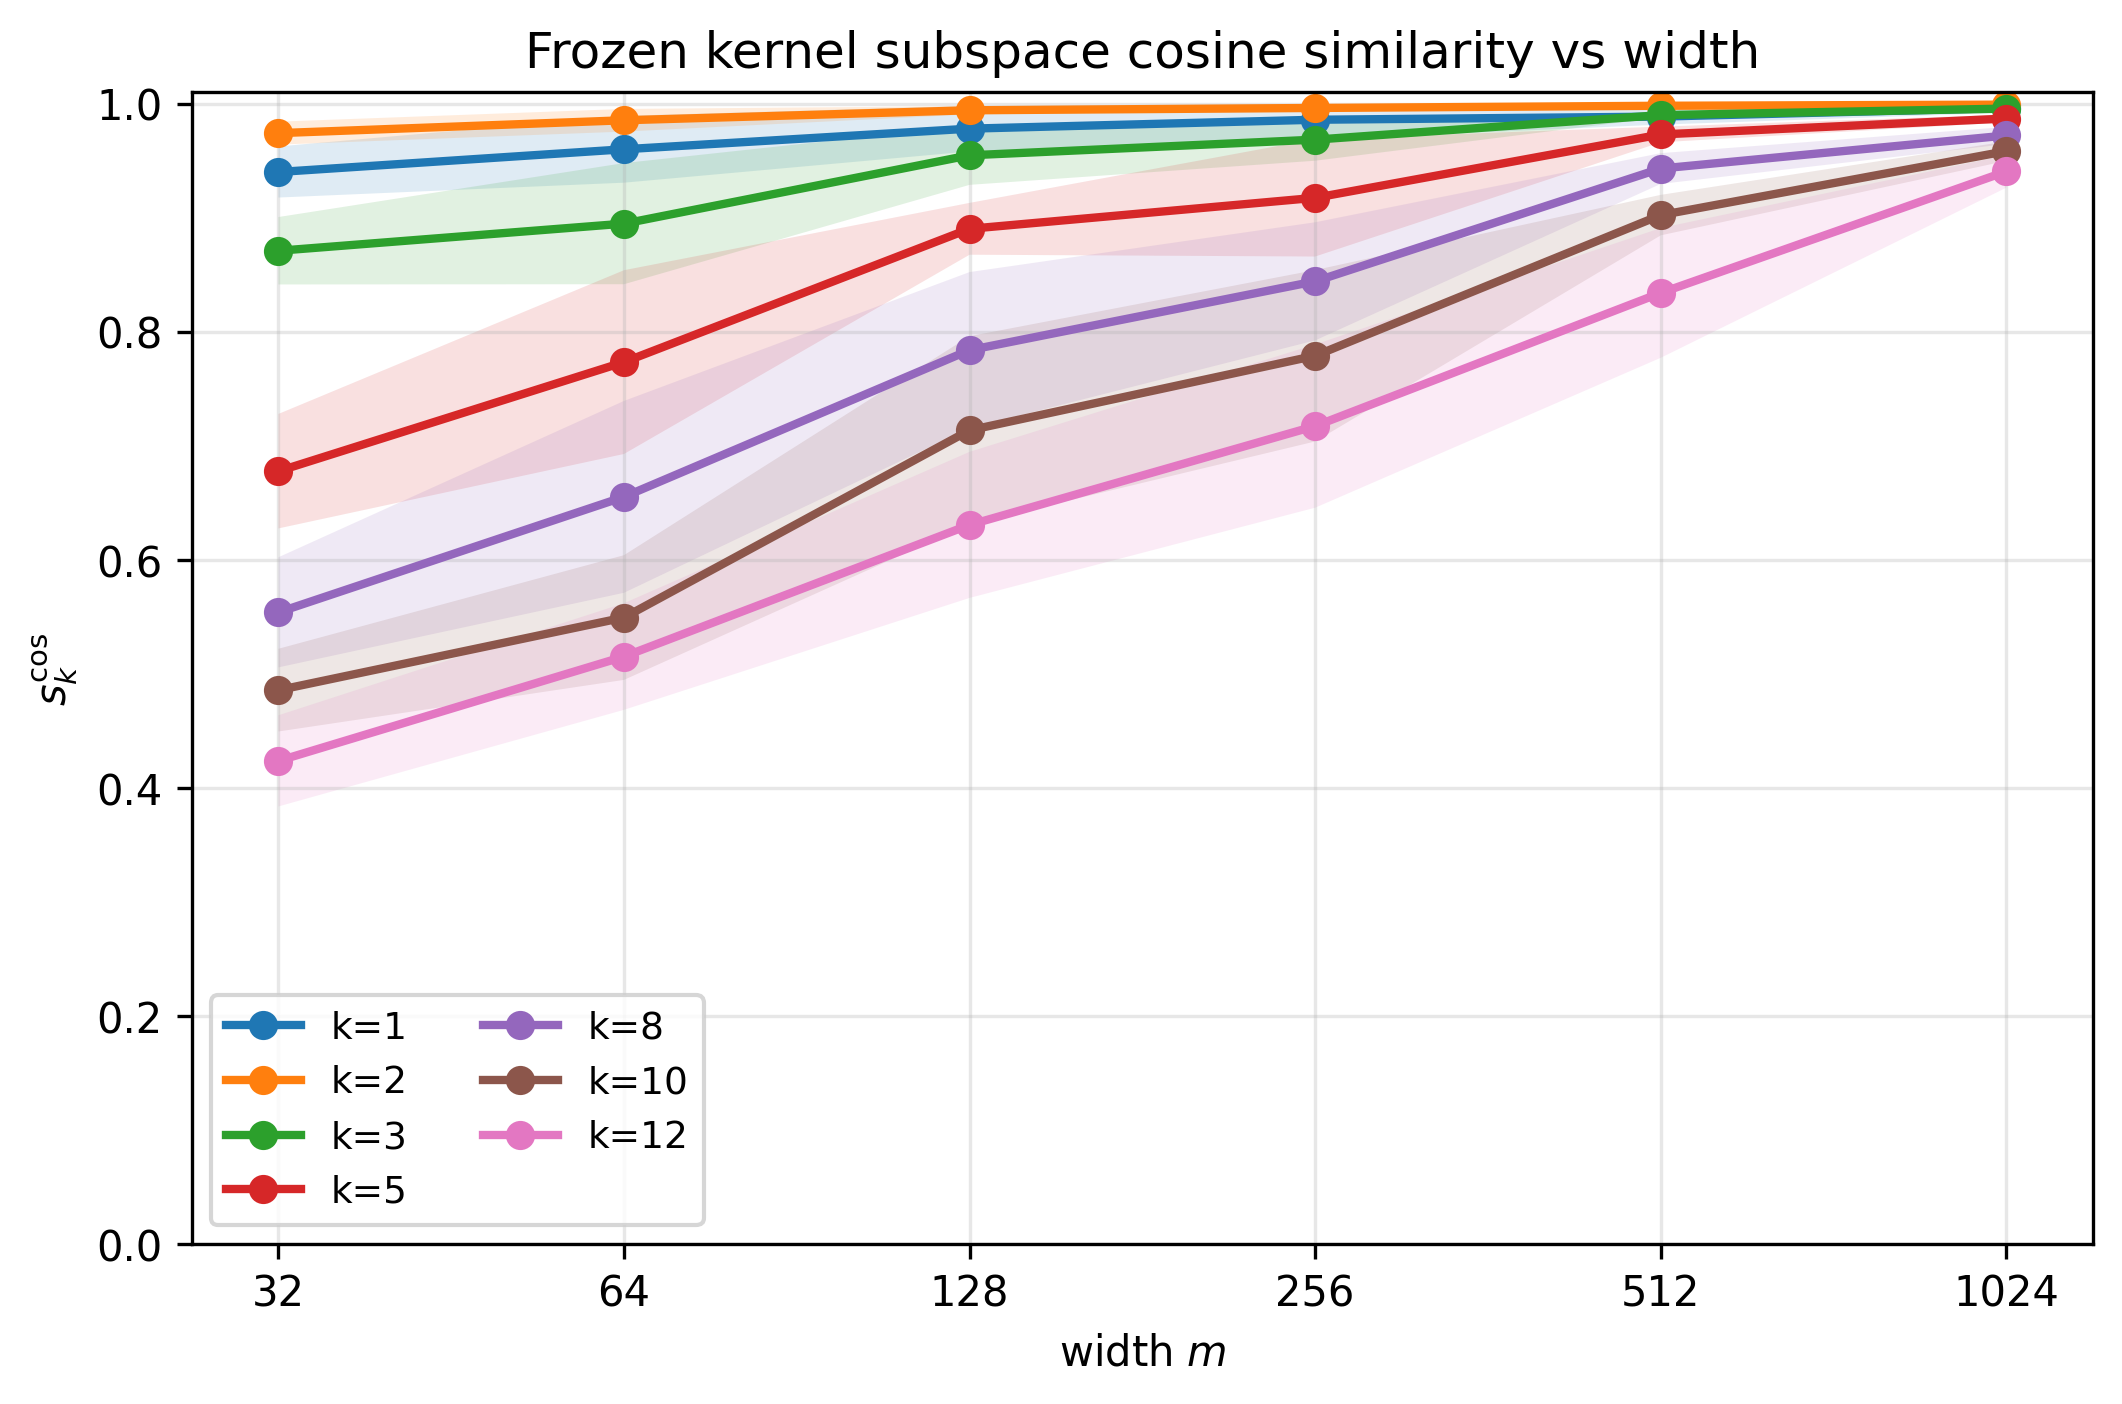
\includegraphics[
				width=\textwidth,
				height=0.78\textheight,
				keepaspectratio
			]{rms_cos_similarity_vs_width}
		\end{column}

	\end{columns}

	\note{
		The key point is that for \(k\ge 1\), cosine and sine have the same continuum eigenvalue,
		so we should compare two-dimensional subspaces rather than individual basis vectors.
		The principal angles measure how well the empirical eigenspace matches the Fourier plane.
		If both angles are small, the two planes are well aligned.
		The cosine similarity aggregates the two angles into a single number between 0 and 1.
		Larger values mean better alignment, and 1 means the empirical eigenspace coincides with the Fourier plane.
		The figure shows that alignment improves with width, and that higher frequencies require larger width.
	}

\end{frame}

\begin{frame}{Finite-width eigenspaces vs Fourier planes}

	\begin{columns}[T,onlytextwidth]

		\begin{column}{0.47\textwidth}
			The two subspaces are both \(2\)-dimensional, so they can be viewed as
			two planes in a high-dimensional space.

			The principal angles
			\[
				0\le \theta_{k,1}\le \theta_{k,2}\le \frac{\pi}{2}
			\]
			measure how well these two planes align.

			We summarize this by the subspace cosine similarity
			\[
				s_k^{\mathrm{cos}}
				=
				\left(
				\frac{1}{2}
				\sum_{i=1}^{2}\cos^2\theta_{k,i}
				\right)^{1/2}.
			\]

			\[
				s_k^{\mathrm{cos}}=1
				\iff
				\widehat{\mathcal F}_k^{(m)}=\mathcal F_k.
			\]
		\end{column}

		\begin{column}{0.51\textwidth}
			\vspace*{1.2cm}
			\centering
			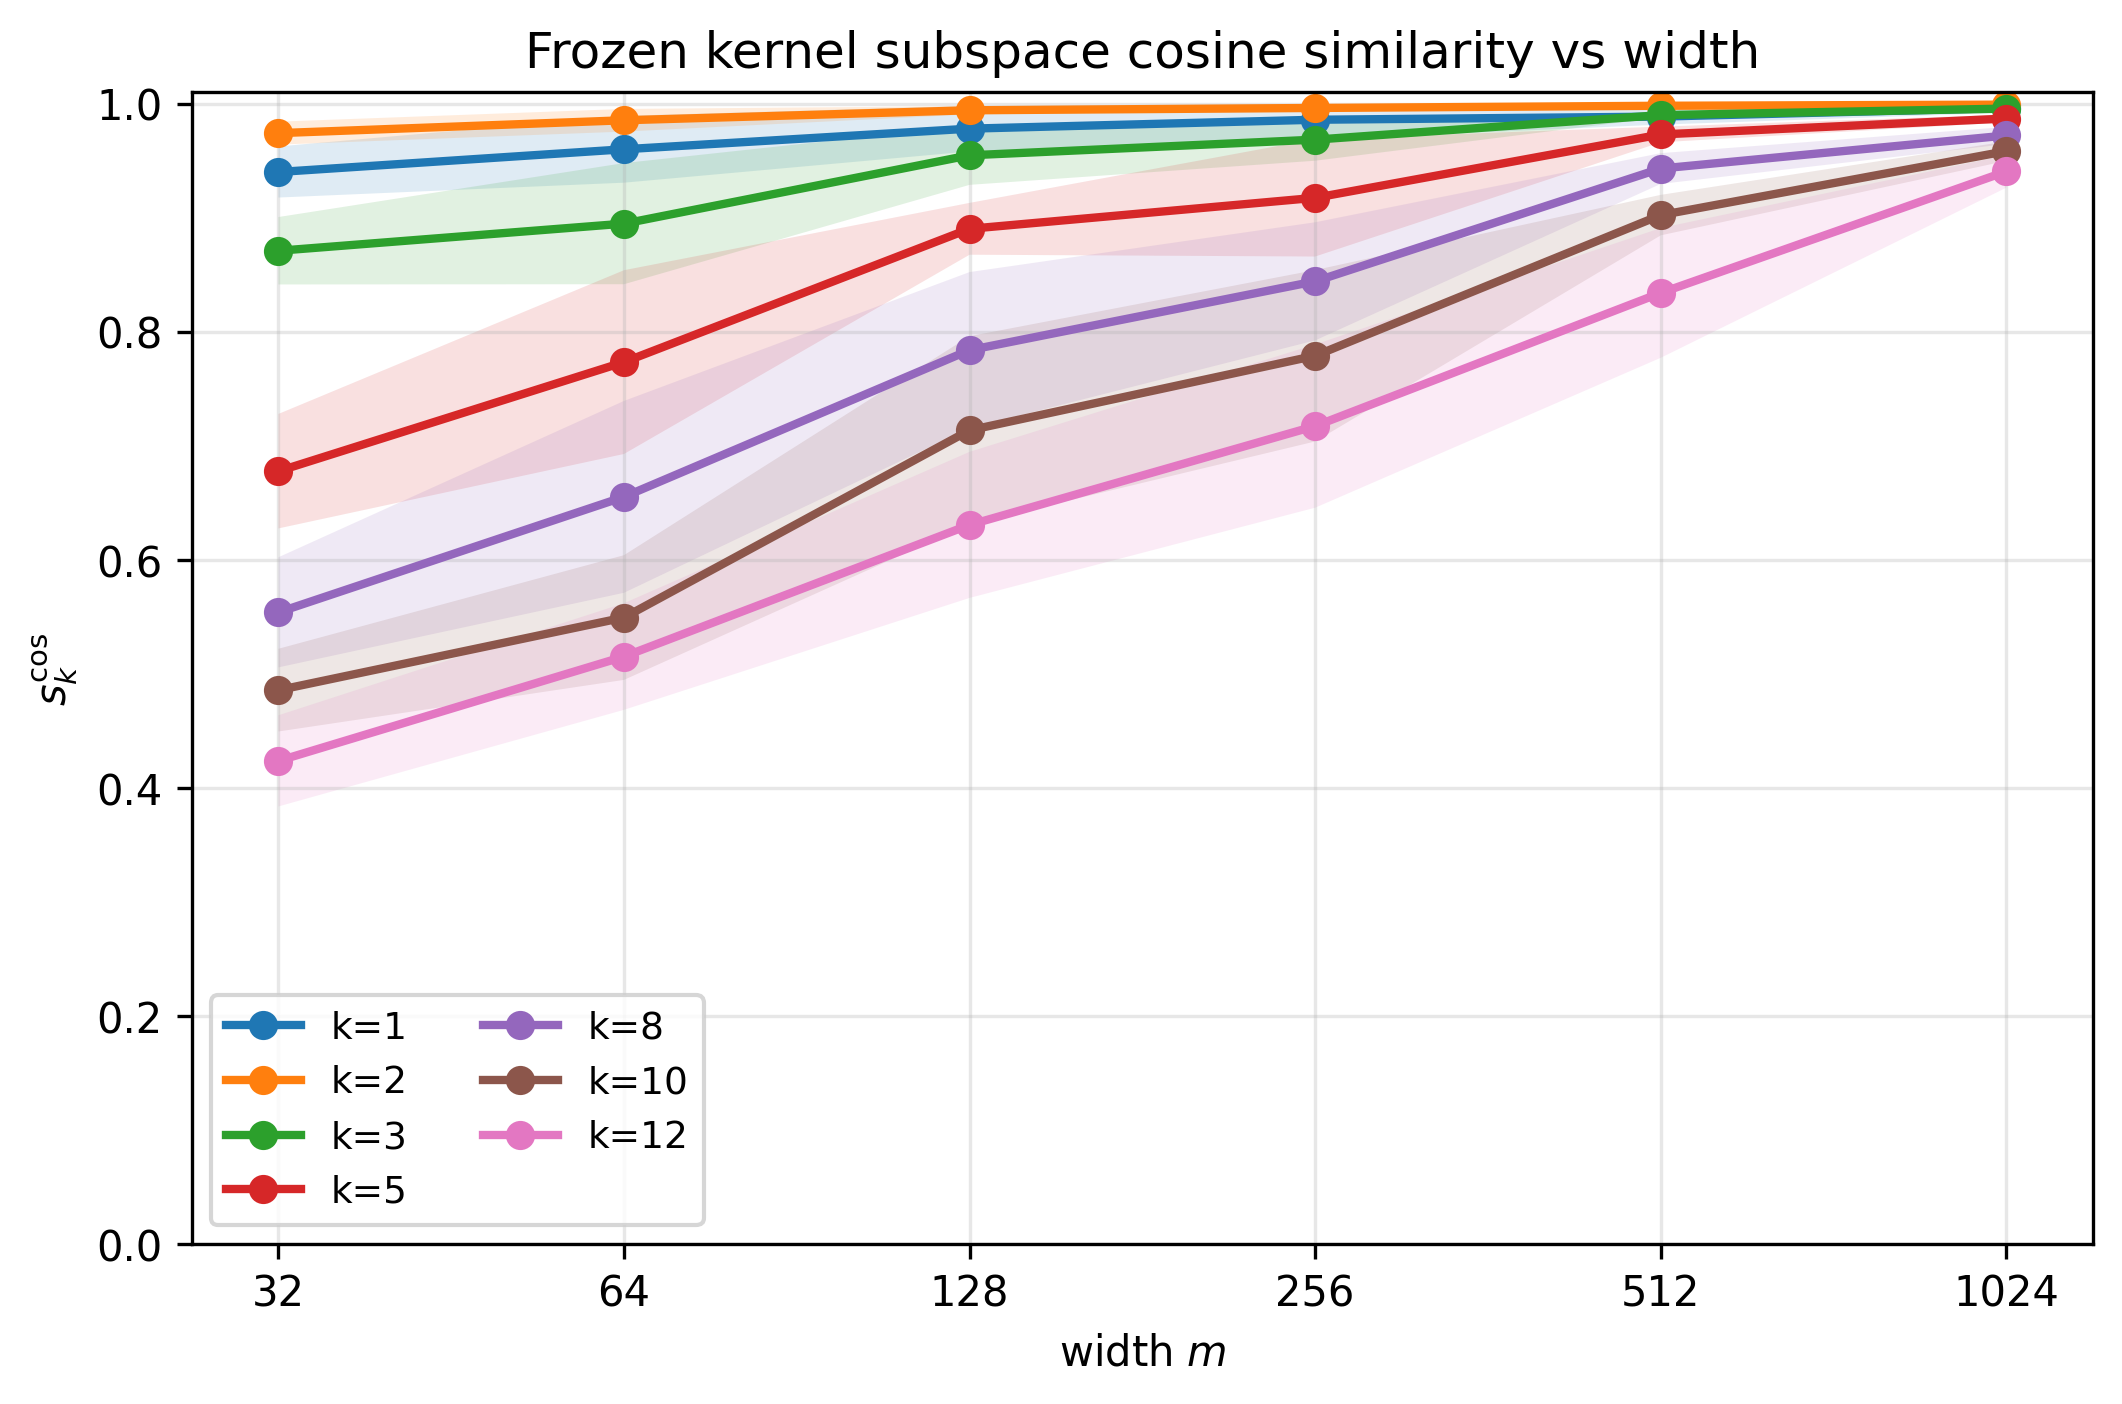
\includegraphics[
				width=\textwidth,
				height=\textheight,
				keepaspectratio
			]{rms_cos_similarity_vs_width}
		\end{column}

	\end{columns}

	\note{
		The key point is that for \(k\ge 1\), cosine and sine have the same continuum eigenvalue,
		so we should compare two-dimensional subspaces rather than individual basis vectors.
		The principal angles measure how well the empirical eigenspace matches the Fourier plane.
		If both angles are small, the two planes are well aligned.
		The cosine similarity aggregates the two angles into a single number between 0 and 1.
		Larger values mean better alignment, and 1 means the empirical eigenspace coincides with the Fourier plane.
		The figure shows that alignment improves with width, and that higher frequencies require larger width.
	}

\end{frame}

\begin{frame}{Frozen versus evolving finite-width dynamics}

	\[
		\text{Frozen: } \frac{d}{dt}r_t=-T_0^{(m)}r_t
		\qquad
		\text{Evolving: } \frac{d}{dt}r_t=-T_t^{(m)}r_t
	\]

	\centering
	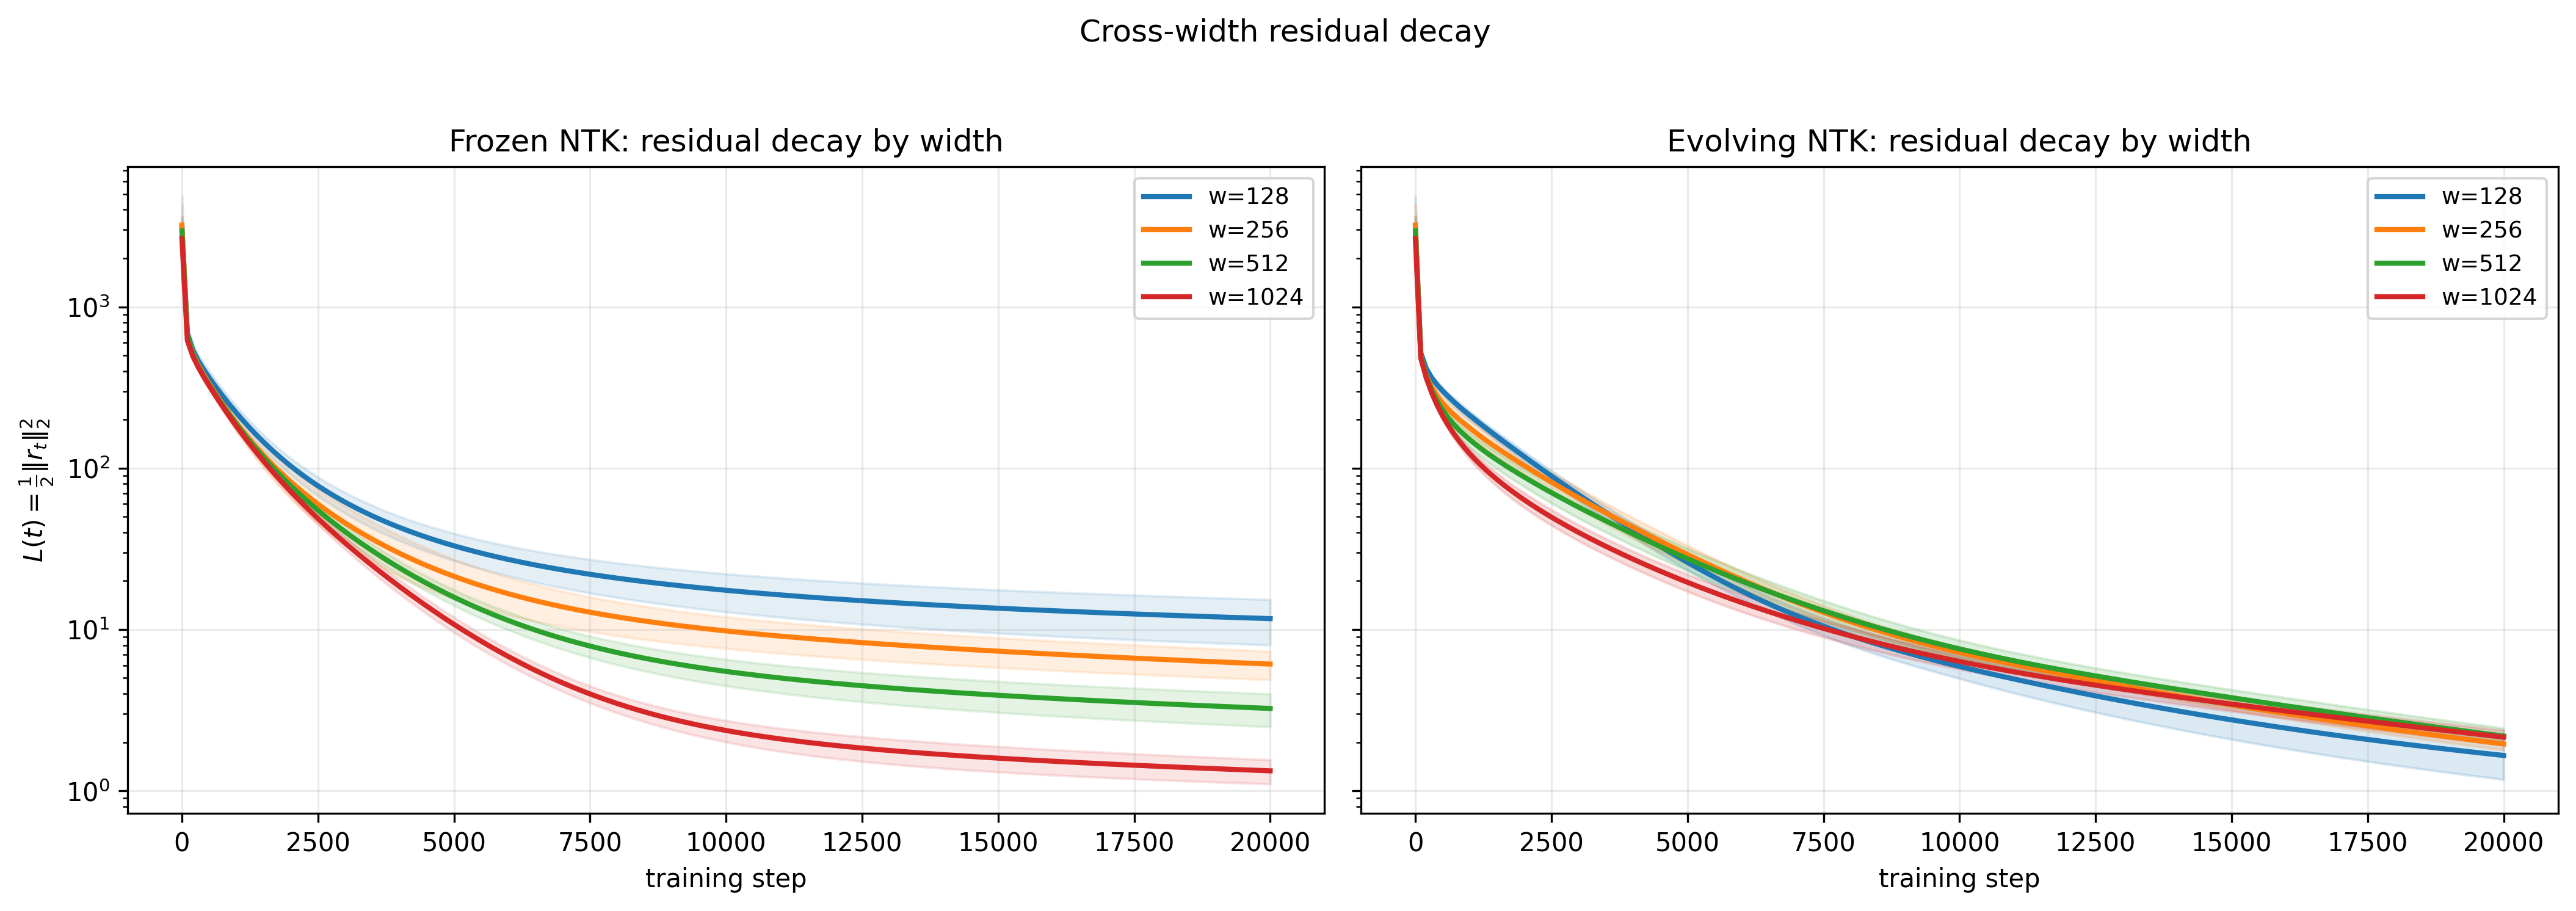
\includegraphics[
		width=0.94\textwidth,
		height=0.68\textheight,
		keepaspectratio
	]{cross_width_residual_decay}

\end{frame}

\begin{frame}{Effect of kernel evolution depends on width}

	\begin{columns}[T,onlytextwidth]

		\begin{column}{0.49\textwidth}
			\centering
			
\includegraphics[
				width=\textwidth,
				height=0.72\textheight,
				keepaspectratio
			]{train_ls_frozen_vs_evolving_w128}
			{\scriptsize Width \(m=128\): evolving kernel reaches lower training error.}
		\end{column}

		\begin{column}{0.49\textwidth}
			\centering
			
\includegraphics[
				width=\textwidth,
				height=0.72\textheight,
				keepaspectratio
			]{train_ls_frozen_vs_evolving_w1024}
			{\scriptsize Width \(m=1024\): frozen kernel performs better.}
		\end{column}

	\end{columns}

	\note{
		At small width, allowing the kernel to evolve gives lower training objective than freezing it at initialization.
		At large width, the frozen kernel is already close to the continuum reference, and the evolving kernel no longer helps in the same way.
		This motivates looking at how kernel evolution changes the Fourier geometry and spectral strength during training.
	}

\end{frame}

\begin{frame}{Does kernel evolution change Fourier alignment?}

	\begin{columns}[T,onlytextwidth]

		\begin{column}{0.49\textwidth}
			\centering
			
\includegraphics[
				width=\textwidth,
				height=0.72\textheight,
				keepaspectratio
			]{rms_cos_alignment_by_freq_w128}

			{\scriptsize Width \(m=128\): stronger loss of alignment for higher frequencies.}
		\end{column}

		\begin{column}{0.49\textwidth}
			\centering
			
\includegraphics[
				width=\textwidth,
				height=0.72\textheight,
				keepaspectratio
			]{rms_cos_alignment_by_freq_w1024}

			{\scriptsize Width \(m=1024\): alignment still degrades, but less severely.}
		\end{column}

	\end{columns}

	\note{
		This slide checks whether the improved optimization performance of the evolving kernel
		comes from better Fourier alignment.

		The dashed curves are the frozen-kernel reference, while the solid curves track the evolving kernel.
		For both widths, higher-frequency Fourier planes lose alignment during training.

		But the effect is not worse at larger width.
		If anything, the larger-width kernel preserves Fourier alignment better:
		the degradation is strongest at width 128 and milder at width 1024.

		So improved training performance at small width is not explained by better subspace alignment.
		That motivates looking next at spectral strength rather than alignment alone.
	}

\end{frame}

\begin{frame}{So why can the evolving kernel perform better?}

	\[
		\mu_{\mathcal F_k}(t)
		=
		\frac{1}{d_k}
		\operatorname{tr}
		\left(
		U_k^\top T_t^{(m)} U_k
		\right)
	\]
	{\small Average kernel strength on the Fourier subspace \(\mathcal F_k\).}

	\vspace{0.15cm}

	\begin{columns}[T,onlytextwidth]

		\begin{column}{0.49\textwidth}
			\centering
			
\includegraphics[
				width=\textwidth,
				height=0.62\textheight,
				keepaspectratio
			]{spectral_strength_by_freq_w128}

			{\scriptsize Width \(m=128\): low-frequency spectral strength increases strongly.}
		\end{column}

		\begin{column}{0.49\textwidth}
			\centering
			
\includegraphics[
				width=\textwidth,
				height=0.62\textheight,
				keepaspectratio
			]{spectral_strength_by_freq_w1024}

			{\scriptsize Width \(m=1024\): spectral strength changes much less.}
		\end{column}

	\end{columns}

	\note{
		The previous slide showed that evolving kernels do not improve Fourier alignment.
		So the better performance at small width must come from something else.

		Here we inspect the average kernel strength on each Fourier subspace.
		This is the trace of the restricted operator divided by the subspace dimension.
		It measures the average effective learning rate available to that frequency subspace.

		At width 128, the evolving kernel substantially increases spectral strength for the low frequencies.
		At width 1024, the same effect is much weaker.
		So at small width, feature learning seems to help by increasing the operator strength on useful low-frequency directions, even though alignment gets worse.
	}

\end{frame}

\begin{frame}{Takeaways}

	\begin{enumerate}
		\item The infinite-width NTK gives a clean Fourier-diagonal reference:
		      \[
			      \frac{d}{dt}r_t=-T_\infty r_t,
			      \qquad
			      T_\infty \phi_p=\lambda_p\phi_p.
		      \]

		\item Finite samples and finite frozen width perturb this picture, but preserve it approximately on \(\mathcal H_K\).

		\item For evolving finite-width networks, the kernel does not simply stay close to the Fourier reference.

		\item At small width, kernel evolution can improve optimization by increasing low-frequency spectral strength, even while Fourier alignment worsens.
	\end{enumerate}

	\vspace{0.25cm}

	\textbf{Main message:}
	spectral bias remains the organizing picture, but finite width changes both the geometry and the effective learning rates.

\end{frame}
\end{document}
